\documentclass{beamer}

\usepackage{amsmath}
% \usepackage{dingbat}
\usepackage{twemojis}
\usepackage{xspace}
\usepackage{multirow}

\input{../../papers/macros/style.tex}
\input{../../papers/macros/primitives.tex}

\def\comring{\ensuremath{\mathsf{comring}}\xspace}
\def\compk{\ensuremath{\mathsf{compk}}\xspace}


\title{Sassafras: Efficient Batch Single Leader Election}

% Semi-anonymous sortition (of) staked assignees (for) fixed-time rhythmic assignment (of) slots

\author{Jeffrey Burdges \and Elizabeth Crites \and Davide Galassi \and \\ Handan Kilinc-Alper \and Alistair Stewart \and Sergey Vasilyev}
\date{ACNS 23-26 June 2025 \\ \vphantom{|} \\ \vphantom{|} \\ \url{https://eprint.iacr.org/2023/031}} % \url{https://eprint.iacr.org/2022/002} \\ \url{https://github.com/w3f/ring-vrf/}}



\begin{document}


\maketitle



% \end{frame}
% \bigskip % \bigskip
% \begin{frame}



\begin{frame}

Distributed systems benefit from leaders election \\ \bigskip\bigskip

Round robin works, but vulneralbe to censorship, etc. \\ \bigskip

Bitcoin is purely a leader election, but proof-of-work sucks.. \\

\end{frame}



\begin{frame}

A \emph{verifiable random function} (VRF) is a signature scheme that proves
evaluation of a pseudo-random function (PRF) determined by the secret signing key.

\bigskip\bigskip

VRFs turn public randomness into secret deterministic randomness, \\ \smallskip
\hspace{10pt}  unlimited reveals after one commit \\

\bigskip\bigskip

VRFs permit sampling with replacement, aka infinite deck games.

\end{frame}



\begin{frame}{Ouroboros Praos}

\begin{center} 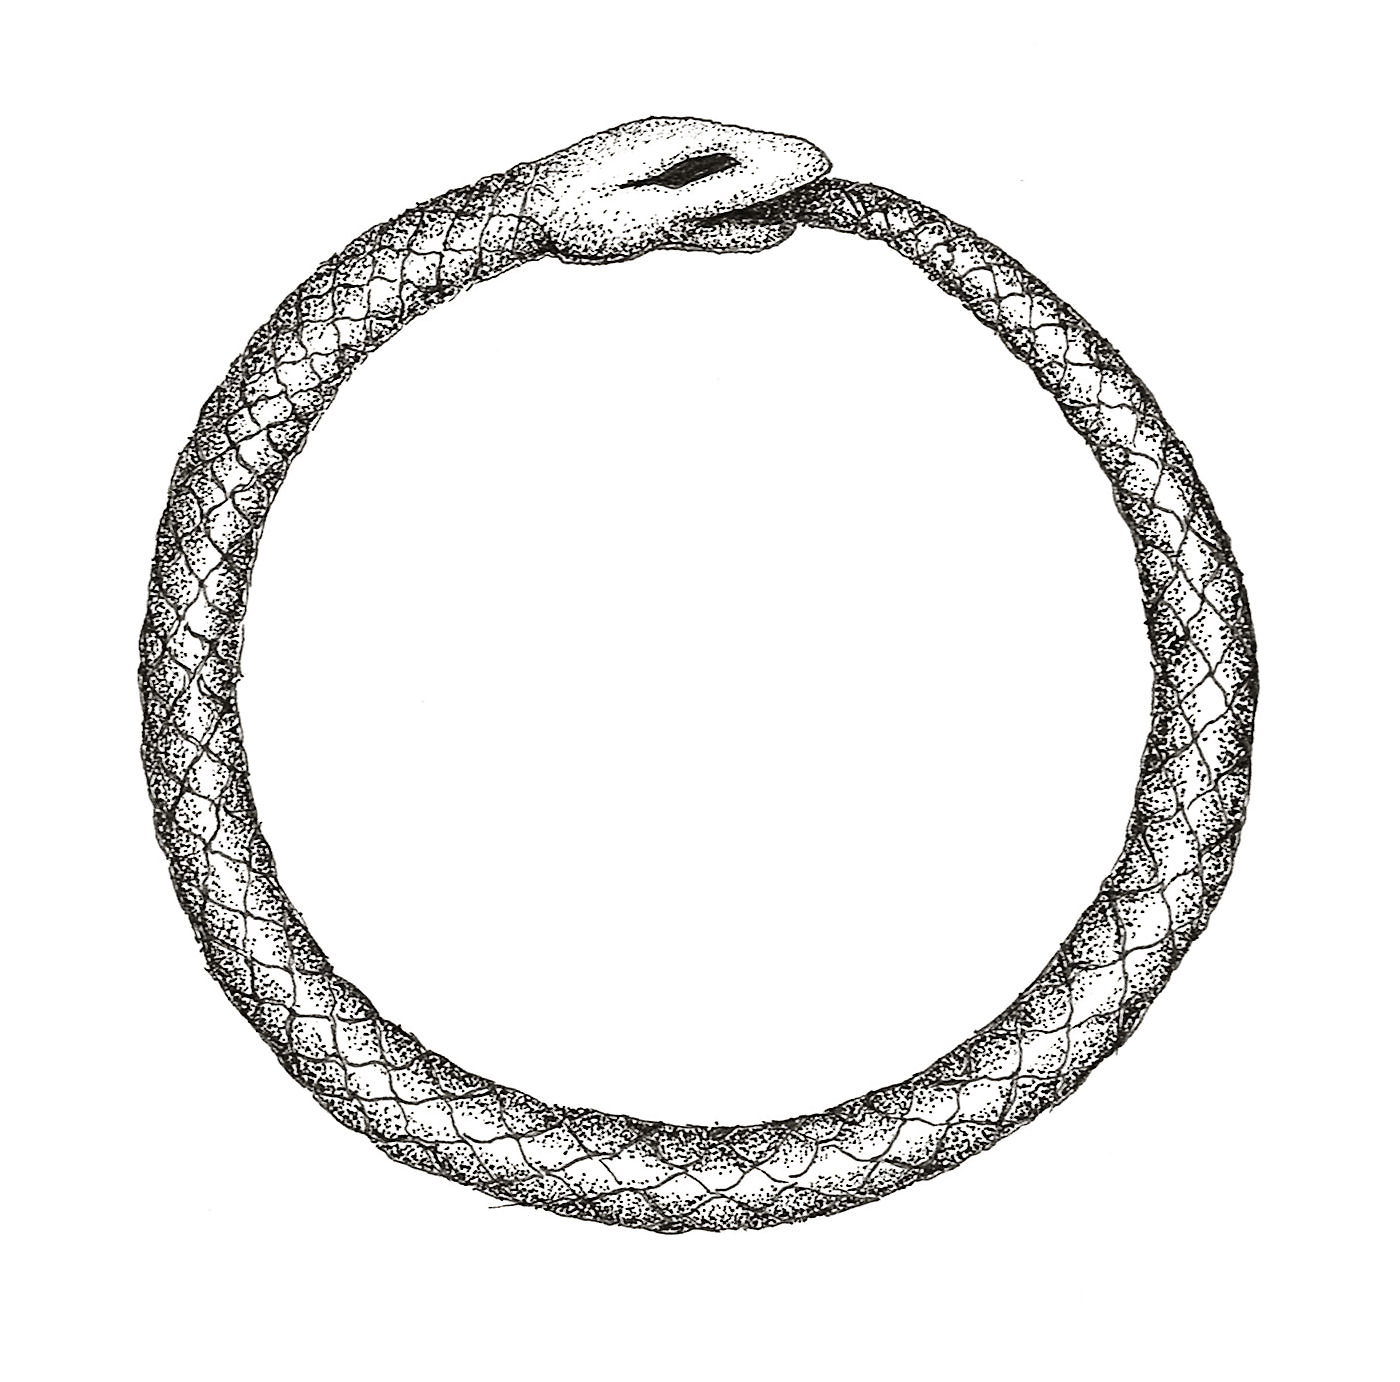
\includegraphics[width=0.8\textwidth]{ouroboros-png-1400.jpg} \end{center}

\end{frame}



\begin{frame}

% VRFs permit sampling with replacement, aka infinite deck games.

\emph{Oroborous Praos} : Almost Bitcoin concensus except.. \\ \smallskip
\hspace{10pt} ``miners'' register VRF keys in advance via stake, \\ \smallskip
\hspace{10pt} replace proof-of-work by a VRF with one input per time slot  \\ \smallskip
\hspace{20pt} and based on some epoch ranodmness, and  \\ \smallskip
\hspace{10pt} epoch randomness is the hash of VRFs from two epochs ago, \\ \smallskip
% \hspace{20pt} which you prove suffices. \\ \smallskip

% \bigskip\medskip

% About like a game of slaps, just like bitcoin. \\ \smallskip
% A batch leader election, but nobody knows when others lead. \\ \medskip

\bigskip\bigskip\medskip

{\bf Problem:}  Praos has unpredictable time between new leaders, which
 creates huge opertunity costs, worsens workflow, etc.

 % \hspace{30pt}  {\color{red} No predictable time between new leaders.}

\end{frame}



\begin{frame}

Secret single leader election (SSLE) means \\ \medskip
\hspace{5pt} new leader every block, only a few seconds appart, and \\ \smallskip
\hspace{5pt} upcoming honest leaders unknown by adversaries.

\end{frame}



\begin{frame}

{\bf Idea:}  Realize SSLEs by a cryptographic shuffle of leaders keys

\bigskip\medskip

{\bf Problem:} Shuffles pass [part of] the deck around the table! \\ \medskip
\hspace{5pt}  The full shuffle needs $O(\mathtt{num\_leaders})$ bandwidth per block. \\ \smallskip
\hspace{5pt}  Secret leaders seems meaningless if $\mathtt{num\_leaders}$ is small. \\ \smallskip
\hspace{5pt}  Reducing this bandwidth reduces anonymity dramatically. \\ \smallskip

% \bigskip\bigskip

% \hspace{20pt} 

\end{frame}



\begin{frame}%{Ring signatures}

Ring signatures prove the actual signer exists in \\
\hspace{10pt} some specified list, known as the ring.

\bigskip\bigskip

Examples: \\
- Some ``deniable'' key exchanges (ugh!). \\
- ZCash \& Monero anonymize payments using ring signatures, \\
\hspace{10pt} avoid double spending using a public log, like eCash.

% $\CommitRing(\ring, \pk_i^?)  \rightarrow (\comring, \openring^?)$ \\
% $\Sign(\sk_i, \comring,\openring, \msg)\rightarrow \sigma$ \\
% $\Verify(\comring,\msg,\sigma) \rightarrow  b$

\end{frame}



\begin{frame}%{Ring signatures}

``Ring'' describes the early linear-time constructions, \\
\hspace{10pt} but now seems anachronistic.

\bigskip\bigskip

$\CommitRing(\ring, \pk_i^?)  \rightarrow (\comring, \openring^?)$ \\
$\Sign(\sk_i, \comring,\openring, \msg)\rightarrow \sigma$ \\
$\Verify(\comring,\msg,\sigma) \rightarrow  b$

\bigskip\bigskip

Asymptotically \& practically far cheaper than shuffles: \\ \smallskip
\hspace{10pt} $O(1)$ verifier and $O(\log |\mathtt{ring}|)$

\end{frame}



\begin{frame}

Ring VRF is a ring signature that's also a VRF.

\bigskip\bigskip 

A ring verifiable random function (ring VRF) is a ring signature that
 proves evaluation of a pseudo-random function (PRF) determined by
 the actual signer's key pair.

\end{frame}



\begin{frame}

Ring VRF is a ring signature that's also a VRF.

\bigskip\bigskip 

$\CommitRing(\ring, \pk_i^?)  \rightarrow (\comring, \openring^?)$ \\
$\mathsf{Eval}(\sk_i, \mathsf{inputs} )\rightarrow \mathsf{outputs}$ \\
$\Sign(\sk_i, \comring,\openring, \msg, \mathsf{inputs} )\rightarrow \sigma$ \\
$\Verify(\comring,\msg, \mathsf{inputs}, \sigma) \rightarrow  (b,\mathsf{outputs})$

\bigskip\bigskip 

Wildy, ring VRFs can be much faster than ring signatures, \\ \smallskip
\hspace{10pt} $O(1)$ verifier and  ``amortized'' $O(1)$ signer!

\end{frame}




\begin{frame}

For what do we use a ring VRF?

\bigskip\bigskip

% black_FRONT050.png

\begin{columns}
        \begin{column}[t]{0.1\textwidth}
        \end{column}
        \begin{column}[t]{0.3\textwidth}
                \includegraphics[width=.9\textwidth]{../images/black_FRONT012.png} % {CAC/PNGs-to-print/individual-cards/black_FRONT012.png}
        \end{column}
        \begin{column}[t]{0.3\textwidth}
                \frame{\includegraphics[width=.9\textwidth]{../images/white_FRONT227.png}} % {CAC/PNGs-to-print/individual-cards/white_FRONT227.png}
        \end{column}
        \begin{column}[t]{0.3\textwidth}
            \frame{\includegraphics[width=.9\textwidth]{../images/white_FRONT117.png}} % {CAC/PNGs-to-print/individual-cards/black_FRONT050.png}
    \end{column}
\end{columns}

\bigskip\bigskip

\url{https://github.com/CardsAgainstBlockchain/}

\end{frame}



\begin{frame}

Cards Against Humanity needs input-output pairs!

\bigskip

Fresh randomness $r$. \\
Set $\mathtt{msgId} = r \doubleplus ``nullifier''$. \\
Set $\mathtt{msgPlay} = r \doubleplus j$ for $j \in \{1,\ldots,5\}$. \\
Publish $\sigma = \mathsf{rVRF}.\Sign(\sk_i,\openring,\mathtt{inId},\mathtt{inPlay})$ \\
or verify $\mathsf{rVRF}.\Verify(\ring_i,\sigma,\mathtt{inId},\mathtt{inPlay})$ \\
Allow each $\mathtt{outId}$ only once, ala nullifier. 
$\mathtt{outPlay}$ determined card played. \\

\bigskip\bigskip

Requires network anonymity layer like Tor.

% Always expect more ``glue'' when hiding anything, ala privacy, etc.

\end{frame}



\begin{frame}{Sassafras}

\includegraphics[width=\textwidth]{../images/Sassafras-albidum.jpg}

\end{frame}



\begin{frame}

Sassafras: Semi-anonymous sortition of staked assignees \\
\hspace{5pt} for fixed-time rhythmic assignment of slots

\bigskip

It's a (semi) secret single leader election (semi-SSLE) \\
\hspace{5pt} by cards against humanity.

\bigskip

% black_FRONT050.png

\begin{columns}
	\begin{column}[t]{0.1\textwidth}
	\end{column}
	\begin{column}[t]{0.3\textwidth}
		\includegraphics[width=.9\textwidth]{../images/black_FRONT012.png} % {CAC/PNGs-to-print/individual-cards/black_FRONT012.png}
	\end{column}
	\begin{column}[t]{0.3\textwidth}
		\frame{\includegraphics[width=.9\textwidth]{../images/white_FRONT227.png}} % {CAC/PNGs-to-print/individual-cards/white_FRONT227.png}
	\end{column}
	\begin{column}[t]{0.3\textwidth}
	    \frame{\includegraphics[width=.9\textwidth]{../images/white_FRONT117.png}} % {CAC/PNGs-to-print/individual-cards/black_FRONT050.png}
    \end{column}
\end{columns}


\end{frame}



\begin{frame}[t]

\emph{Sassafras} : Semi-SSLE by cards against humanity \\ \bigskip\bigskip

\hspace{5pt} Assume $\alpha < 1/3$ Byzantine participants. \\ \medskip

\hspace{5pt} Collect epoch randomness from an earlier epoch like Paros, \\ 
\hspace{15pt} so using a regular VRF. \\ \medskip

\hspace{5pt} Create an anonymous schedule in an earlier epcoh too, \\ 
\hspace{15pt} using a ring VRF plus a network anonymity layer. \\ \medskip

\hspace{5pt} Claim the scheduled ``tickets'' using a regular VRF but \\ 
\hspace{15pt} that evaluates exactly like our ring VRF. \\

\end{frame}



\begin{frame}[t]


\hspace{30pt} \emph{Anonymous scheduling} \\ \bigskip % in Sassafras

Fix $n$ candidate leaders and $m$ slots per epoch. \\ \smallskip

\emph{Compute tickets} : \\
\hspace{15pt} Define $t \gg m/n$ inputs based upon epoch randomness. \\ \smallskip
\hspace{15pt} Evaluate the outputs for these $t$ intputs. \\ \smallskip
\hspace{15pt} Keep only ``good'' outputs, say hash smaller than $2 m \over t n$.  \\ \smallskip
\hspace{15pt} Compute a ring VRF ticket for good input-output pairs. \\ \bigskip

\emph{1-hop anonymity layer} : \\
\hspace{5pt} Send your good tickets to a random other ``repeater'' peer. \\ \smallskip
\hspace{5pt} Repeaters publish any valid tickets they recieve. \\ \smallskip
\hspace{5pt} If a repeater drops your ticket then publish it yourself. \\ \bigskip

\emph{Compute schedule} : \\
\hspace{5pt} Chain sorts the tickets and drop the middle so only $m$ remain. \\ \bigskip

\end{frame}



\begin{frame}[t]

\hspace{30pt} \emph{Using the schedule} \\ \bigskip

\emph{Ellection} : \\
\hspace{5pt} Claim your leader slot scheduled two epoch ago using  \\
\hspace{15pt} a regular VRF that evaluates like the ticket ring VRF.  \\ \smallskip
\hspace{5pt} Attach to blocks an independent block VRF for randomness. \\ \bigskip

\emph{Epoch randomness} : \\
\hspace{5pt} Hash all block VRFs from four epochs ago. \\ \bigskip

% \bigskip\bigskip

% Although imperfect, Praos gives a nice cheap randomness source, which can be analyized

\end{frame}



\begin{frame}

% - Network layer anonymity is weak, which requires analysis. \\
% - Vastly more efficient than Boneh's shuffle SSLEs or WHISK \\ \smallskip

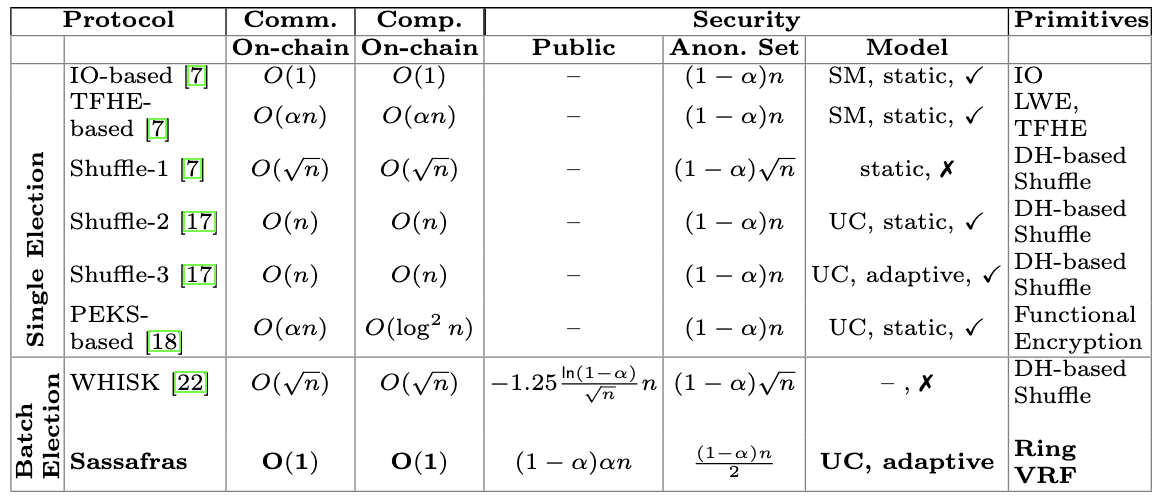
\includegraphics[width=\textwidth]{related_work.png}

\bigskip

Anonymity sets: $(1-\alpha) \sqrt{n}$ in WHISK vs ${1-\alpha \over 2} n$ in Sassafras (pp. 5) \\ \bigskip

A shuffle optimized for bandwidth leaves only small anonymity sets \\
\hspace{5pt}  so all honest leaders could be weakly corrupted aka DoSed.

\end{frame}




\begin{frame}%{Sassafras}

Variations: \\ \medskip
- Improve network anonymity layer, which requires more fallbacks \\ \medskip
- Block producers can prove their slot in advance \\ \medskip
% - Users send tx to upcoming slots via Tor-like {.onion} circuits. \\ \smallskip
- Add per-ticket Tor {.onion} URLs into the tickets,  \\ \smallskip
\hspace{5pt} so users can sent tx to upcoming leaders more. \\ \smallskip
\hspace{5pt} Avoiding memepools saving 50\% bandwidth and 50\%-99\% CPU. \\ \smallskip
\hspace{5pt} Allows better MEV defenses? \\ \medskip
- Leaders keep Tor-like anonymity after making their block \\

\end{frame}







\begin{frame}{Identity using ring VRFs}

Ring consists of people, with one key per person, \\ 
\hspace{10pt} maybe populated from government identity documents.

\bigskip\smallskip

User agent: \\ \smallskip

1st) validates TLS cert of ``site.com'', including CT logs. \\ \smallskip

2nd) sends ring VRF signature with $\msg = \mathtt{``site.com``}$. \\ \smallskip

% \pause\bigskip\bigskip 
% 
% Do we have a ``right to be forgotten'' at ``site.com``? \\ \smallskip
% 
% \hspace{10pt} If so, use $\msg = \mathtt{``site.com``} \doubleplus \mathsf{month}$

\bigskip\bigskip 

Anonymous rationing uses $\msg = \mathtt{``moutarde``} \doubleplus \mathsf{week} \doubleplus \mathsf{counter}$ \\
\hspace{1pt} And treats outputs as short lived nullifiers.

\bigskip 

Also yields free-to-play games, promotional discounts, etc.

\end{frame}



\begin{frame}

Identity by attribute based credentials: \bigskip

- Authorities issue fraudulent certificates, ala CAs and Covid. \\ \smallskip
- Attributes are unecessarily invasive. \\ \smallskip
- Attributes leak across domains.  Users cannot change attributes. \\ \smallskip
- Users make mistakes and/or can be forced. \\ \medskip
\hspace{30pt}  {\color{red} Attribute requests need certificate infrastructure}

\bigskip\smallskip

Identity by ring VRFs: \\ \smallskip

- Rate limits! \\ \smallskip
- Issuance ``only'' requires uniqueness or mearly limitations \\ \smallskip
- Nothing leaks if properly domain seperated \\ \smallskip
\hspace{30pt}  {\color{green}  Can avoids certificate infrastructure}

\end{frame}


\begin{frame}
 
``No civilization can possibly survive to an interstellar spacefaring \\ \smallskip
\hspace{1pt} phase unless it limits its numbers'' (and its consumption) \\ \medskip
\hspace{1pt} --- Carl Sagan

\bigskip\bigskip 

We're headed for $+4^{\circ}$C by 2100, so uninhabitable tropics \\
\hspace{10pt} and world carrying capacity below 1 billion people (Steffan). \\ \bigskip

50\% odds ``of a synchronous crop failure [$>10$\%] across all four [major maize producing] countries during 2040s''~(Chatham~House) \\

\end{frame}







\begin{frame}{Zero-knowledge in substrate?}

Yes WASM works, but 10x slower for some optimized code.

\bigskip \bigskip

EIP-2537 (BLS12-381) adds 9 precompiles (hostcalls).  
{\Large\twemoji{thumbs down}}
% \includegraphics[width=0.03\textwidth]{../images/thumbs_down.png}
\\ \medskip

\only<1>{
\hspace{5pt} Extra complexity means fewer curves \\
\hspace{10pt}- Addition \& hash-to-curve appear unecessary. \\ \medskip

\hspace{5pt} Inflexibility yields worse performance  \\ 
\hspace{10pt}- Groth16 needs 4 pairings \\
\hspace{10pt}- Batch verifiers \\
\hspace{10pt}- Large parameters like KZG trusted setups \\
}
\bigskip\bigskip
\only<2>{
Add hostcalls for the "slow parts" but use WASM elsewhere
{\Large\twemoji{thumbs up}}
% \includegraphics[width=0.03\textwidth]{../images/thumbs_up.png}
\\ \smallskip

\hspace{5pt} Bandersnatch, etc. --- single \& multi-scalar multiplication \\

\hspace{5pt} BLS12-381, BLS12-377, BW6-761, BW6-767, BN254 --- \\
\hspace{10pt}  Same, plus multi-miller loop \& final exponentiation \\ \smallskip
}

\bigskip \bigskip 

\url{https://github.com/paritytech/arkworks-extensions}
\end{frame}


\begin{frame}

Arkworks \& others mostly descend from Zcash. \\ \smallskip

Adapt crates directly, without reimplementation.

\smallskip

\includegraphics[width=0.9\textwidth]{../images/use_curves.png}

\url{https://github.com/paritytech/arkworks-extensions}

\end{frame}


\end{document}




















\begin{frame}
		
\end{frame}



\begin{frame}
	
\end{frame}














% \begin{table}[t]
	\centering
	\scriptsize
	\begin{tabular}{|c|m{1.6cm}|c|c|c|c|c|m{1.4cm}|}
			\hline
		\multicolumn{2}{|c|}{\textbf{Protocol}}&{\textbf{Comm.}}&{\textbf{Comp.}}&\multicolumn{3}{|c|}{\textbf{Security}} & \textbf{Primitives} \\
\arrayrulecolor{gray}% requires \usepackage{colortbl}
\hline
		&&\textbf{On-chain} &\textbf{On-chain}& \textbf{Public}&\textbf{Anon. Set} & \textbf{Model} &\\
		\hline
		\multirow{6}{*}{\rotatebox[origin=c]{90}{\parbox[c]{3cm}{\textbf{Single Election}}}}&IO-based \cite{singleleader}  & $ O(1) $ &$ O(1) $& --&$ (1-\alpha) n $  & SM, static, \checkmark &  IO\\
%		\hline
		&TFHE-based~\nocite{singleleader} & $ O(\alpha n) $ &$ O(\alpha n) $&--& $ (1-\alpha) n $ & SM, static, \checkmark & LWE, TFHE\\
%		\hline
%		Shuffle-based (1)\cite{singleleader} & $ O(n) $ &1&1& $ \frac{1}{n-m} $ & Shuffle &SM, static\\ 
%		\hline
		&Shuffle-1 \nocite{singleleader} & $ O(\sqrt{n}) $ &$ O(\sqrt{n}) $&-- & $(1-\alpha) \sqrt{n}$& static, \ding{55} & DH-based Shuffle \\
		&Shuffle-2 \nocite{ssle-adaptive} & $ O(n) $  & $ O(n) $  & -- & $ (1-\alpha) n$ &UC, static, \checkmark & DH-based Shuffle\\
		
		&Shuffle-3 \nocite{ssle-adaptive} & $ O(n) $ & $ O(n) $  & -- & $ (1-\alpha) n $ & UC, adaptive, \checkmark &DH-based Shuffle\\
		
		&PEKS-based~\nocite{ssleUC}& $ O(\alpha n) $ &$ O(\log^2 n)$& --& $ (1-\alpha) n $ &  UC, static, \checkmark & Functional Encryption\\
		\hline
	
		\multirow{2}{*}{\rotatebox[origin=c]{90}{\parbox[c]{1.15cm}{\textbf{Batch  Election}}}}&WHISK \cite{whisk} & $ O(\sqrt{n}) $  &$ O(\sqrt{n}) $ & $ -1.25\frac{\mathsf{ln}(1-\alpha)}{\sqrt{n}} n$ & $ (1-\alpha) \sqrt{n} $ & -- , \ding{55} &DH-based Shuffle\\
		& & & & & & &\\
		&\textbf{Sassafras } & $ \mathbf{O(1)} $ & $ \mathbf{O(1)} $  & $ (1-\alpha) \alpha n$ & $\frac{(1-\alpha)n}{2}$ & \textbf{UC, adaptive} & \textbf{Ring VRF}\\
		
%		\hline
%		\cite{ssleUC} (optimized) & $ O(\log^2n ) $ &$ 4$&1& $ \frac{1}{n-m} $ & PEKS & UC, static\\
%		\hline
%			\cite{ssle-adaptive} & $ O(n) $ &$ 1$?&1& $ \frac{1}{n-m} $ & Shuffle & UC, adaptive\\
%		\hline
%		SASLE (Ours) & $ O(n) $ &2&$ \eplen \geq 1 $ &$ \approx  \frac{1}{n-m}  $ for $ (1-\alpha)\eplen $ elections in expectation & Ring VRF&UC, adaptive\\
		\hline
	\end{tabular}
%	\vspace{.3cm}
% \caption{\scriptsize Single secret leader election (SSLE) protocols. $ n $ is the total number of participants, $ \alpha $ is the fraction of corrupt parties, and $(1-\alpha)$ is the fraction of honest parties. 
% Batch Election refers to running $\ell$ elections at once, and values are given per election.
% Comm. and Comp. are communication and computational complexity, respectively.
% Public is the 
% %expected number of non-secret single leaders in  $ \ell $-elections where $ 1 \leq \ell \leq n $. 
% fraction of leaders in a batch election that are leaked, 
% and the unpredictability level of a leader (Definition~\ref{def:unpredictability}) is the reciprocal, e.g., $\frac{1}{(1-\alpha) \sqrt{n}}$.
% For Sassafras, this is calculated in Proposition~\ref{prop:parameter}.
% SM is the Standard Model and UC is the Universal Composability model. 
% \ding{55} means the protocol is insecure under our threat model, as described below; \checkmark means it is secure in our model.
% The security model for WHISK~\cite{whisk} is marked `--' because no formal security analysis is provided.  Other terms are defined below.}
% \vspace{-.3cm}
% \hrulefill
% \vspace{-.5cm}
% \label{tbl:comparison}
% \end{table}